First of all, let us examine what an antibody is, and see how this
type of molecules possesses remarkable properties that make it suitable
for therapeutic use.

An antibody (also known as Immunoglobulin) is a protein produced by the 
body's immune system that binds to a specific antigen. It is composed of four
polypeptide chains: two identical heavy chains 
and two identical light chains \cite{davies_antibody_1993}. 

The way this chains are self-assembled gives the protein a Y-shaped structure. 
Each of them possesses a terminal high-variability domain, which when grouped spatially
together forms a binding site that can be adapted to a wide variety of antigens.

\begin{figure}[H]
    \begin{minipage}{0.495\textwidth}
        \centering
        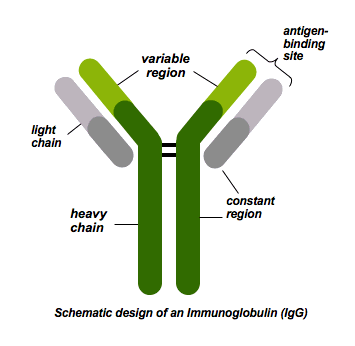
\includegraphics[width=0.8\textwidth]{../Images/schematics_antibody.png}
        \caption{Schematic representation of an antibody} 
        \label{fig:schematics_antibody}
    \end{minipage}\hfill
    \begin{minipage}{0.495\textwidth}
        \centering
        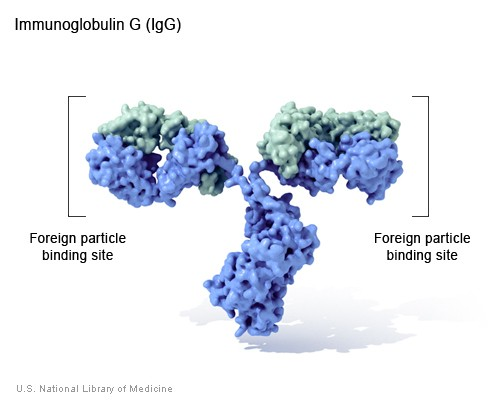
\includegraphics[width=0.8\textwidth]{../Images/immunoglobulin_3D_model.jpg}   
        \caption{3D model of an antibody}
        \label{fig:immunoglobulin_3D_model}
    \end{minipage}
\end{figure}


\begin{figure}[H]
    \begin{minipage}{0.6\textwidth}
        The variation between immunoglobulins in the low-variability domain
        creates multiple antibody classes, also known as \emph{isotypes} :
        IgA, IgD, IgE, IgG, or IgM. They all have different functions, but act
        following the same general principles that will be discussed later in this paper.

        The most important one are :
        \begin{itemize}[leftmargin=*]
            \item IgG, which represents $75\%$ of serum antibodies
            in humans. It is involved in the immunity transmitted by a mother
            to her newborn, protecting the child for the first six months of life
            before it can acquire its own immune memory.
            \item IgM, which auto-assembles to form a pentamer, is the largest
            antibody and one of the first to response to an antigen intrusion.
        \end{itemize}
    \end{minipage}\hfill
    \begin{minipage}{0.35\textwidth}
        \centering
        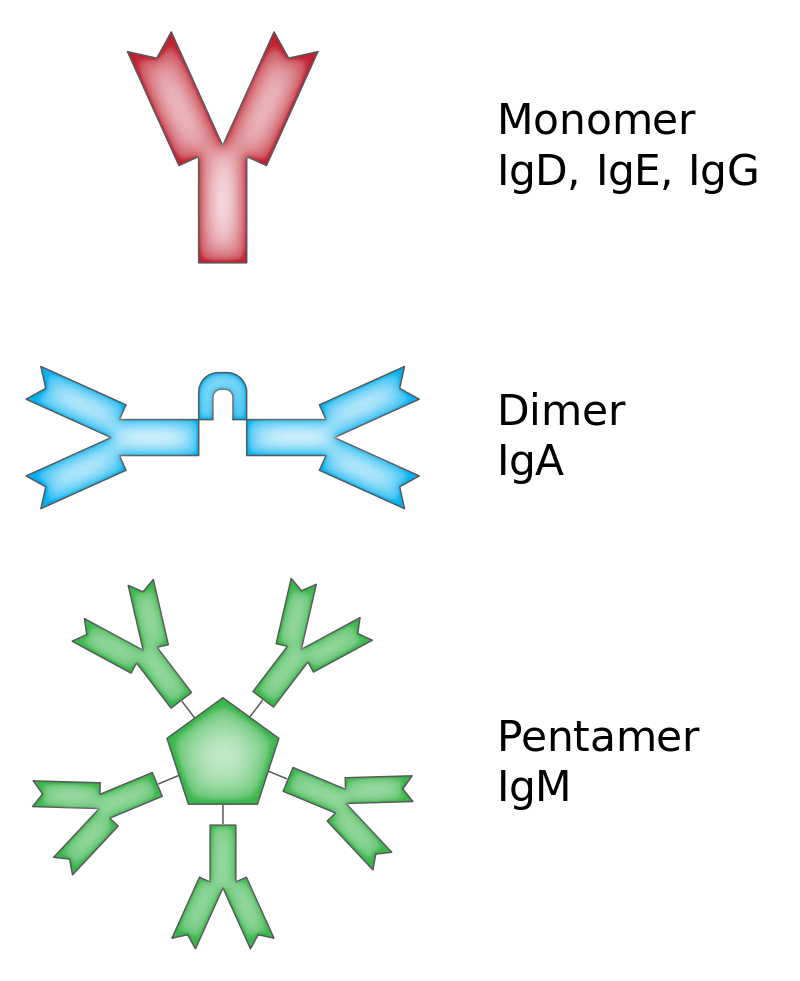
\includegraphics[width=\textwidth]{../Images/antibody_classes.png}   
        \caption{The different antibody isotypes and the way they naturally polymerize}
        \label{fig:antibody_classes}
    \end{minipage}
\end{figure}
